\documentclass[11pt]{article}
\usepackage[left= 1.55cm, right = 1.55cm,top = 1.2cm, bottom = 1.5cm]{geometry}
\usepackage{enumerate}
\usepackage{amsmath,amsfonts,amssymb}
\usepackage{setspace}
\usepackage{float}
\usepackage{multicol}
\usepackage{xcolor}
\usepackage[hidelinks]{hyperref}
\usepackage{listings}
\definecolor{codegreen}{rgb}{0,0.6,0}
\definecolor{codegray}{rgb}{0.5,0.5,0.5}
\definecolor{codepurple}{rgb}{0.58,0,0.82}
\definecolor{backcolour}{rgb}{0.95,0.95,0.92}
\lstdefinestyle{mystyle}{
    backgroundcolor=\color{backcolour},   
    commentstyle=\color{codegreen},
    keywordstyle=\color{magenta},
    numberstyle=\tiny\color{codegray},
    stringstyle=\color{codepurple},
    basicstyle=\ttfamily\footnotesize,
    breakatwhitespace=false,         
    breaklines=true,                 
    captionpos=b,                    
    keepspaces=true,                 
    numbers=left,                    
    numbersep=5pt,                  
    showspaces=false,                
    showstringspaces=false,
    showtabs=false,                  
    tabsize=2
}
\lstset{style=mystyle}
\pagenumbering{gobble}
\renewcommand{\arraystretch}{1.5}
\usepackage{mathtools}
\usepackage{longtable}
\usepackage{graphicx}
\usepackage{multirow}
\usepackage{hhline}
\usepackage[utf8]{inputenc}
\usepackage[usestackEOL]{stackengine}
\setlength{\abovedisplayskip}{0in}
\setlength{\columnsep}{3em}
\newcommand{\blue}{\color{Blue}}
\newcommand{\green}{\color{Green}}
\usepackage[inkscapeformat=png]{svg}
\newcommand{\red}{\color{Red}}
\newcommand{\black}{\color{Black}}
\newcommand{\Name}{Communities }
\title{Software Requirements Analysis\\ Online Social Media Platform\\ SM02\\Grouup 9}
\author{Harshit Pant \\ CS21BTECH11021 \and Satpute Aniket Tukaram \\ CS21BTECH11056 \and Mahin Bansal \\ CS21BTECH11034 \and Burra Vishal Mathews \\ CS21BTECH11010}
\date{}
\begin{document}
\maketitle
\begin{center}
    \tableofcontents
\end{center}
\section{Context Diagram}

\begin{figure}[H]
    \centering
    \makebox[\linewidth][c]{\hspace{5cm}
        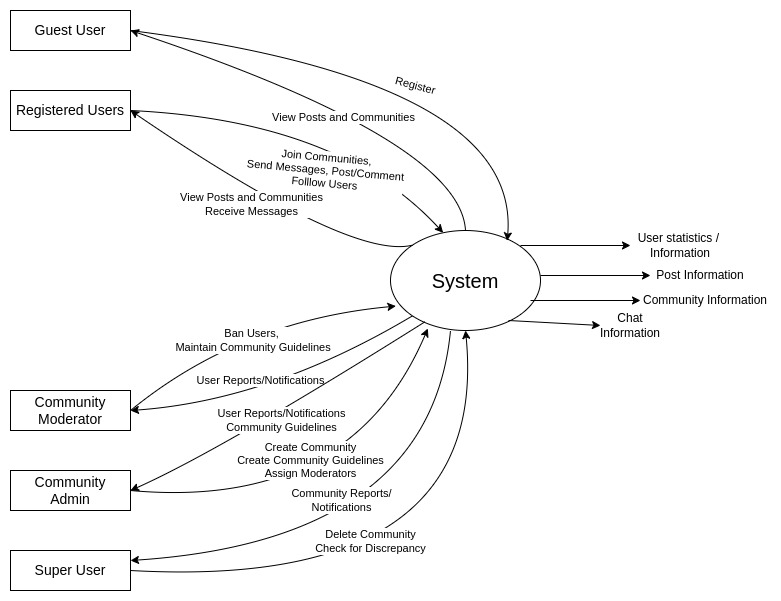
\includegraphics[width = 0.75\textwidth]{./images/context_diagram.jpeg}
    }
    \caption{Context Diagram}
    \label{fig:context_diagram}
\end{figure}

\begin{itemize}
    \item \textbf{Actors : } There are 5 Roles in this environment.
    \item \textbf{Guest User }interacts with the system by registering and viewing posts and communities
    \item \textbf{Registered User }interacts with the system by joining different communities, sending Messages to other registered users creating posts for communitities, commenting on posts, following users
          and viewing posts,viewing communities, receiving messages from other users
    \item \textbf{Community Moderators }interact with system by banning users in that community, deleting comments and posts to maintaining community guidelines and receive user reports and notifications
    \item \textbf{Community Admin }interacts with system by creating communities, creating community guidelines, assigning moderators and receives reports and notifications
    \item \textbf{Super User} interacts with the system by Deleting Communities,Checking for Discrepancy and receives community reports and notifications
    \item \textbf{System }provides user statistics, post information, community statistics and chat information
\end{itemize}

\section{Data Flow Diagrams}
\subsection{DFD Descriptions}
Below are two possible DFDs for the system.
\begin{figure}[H]
    \centering
    \makebox[\linewidth][c]{
        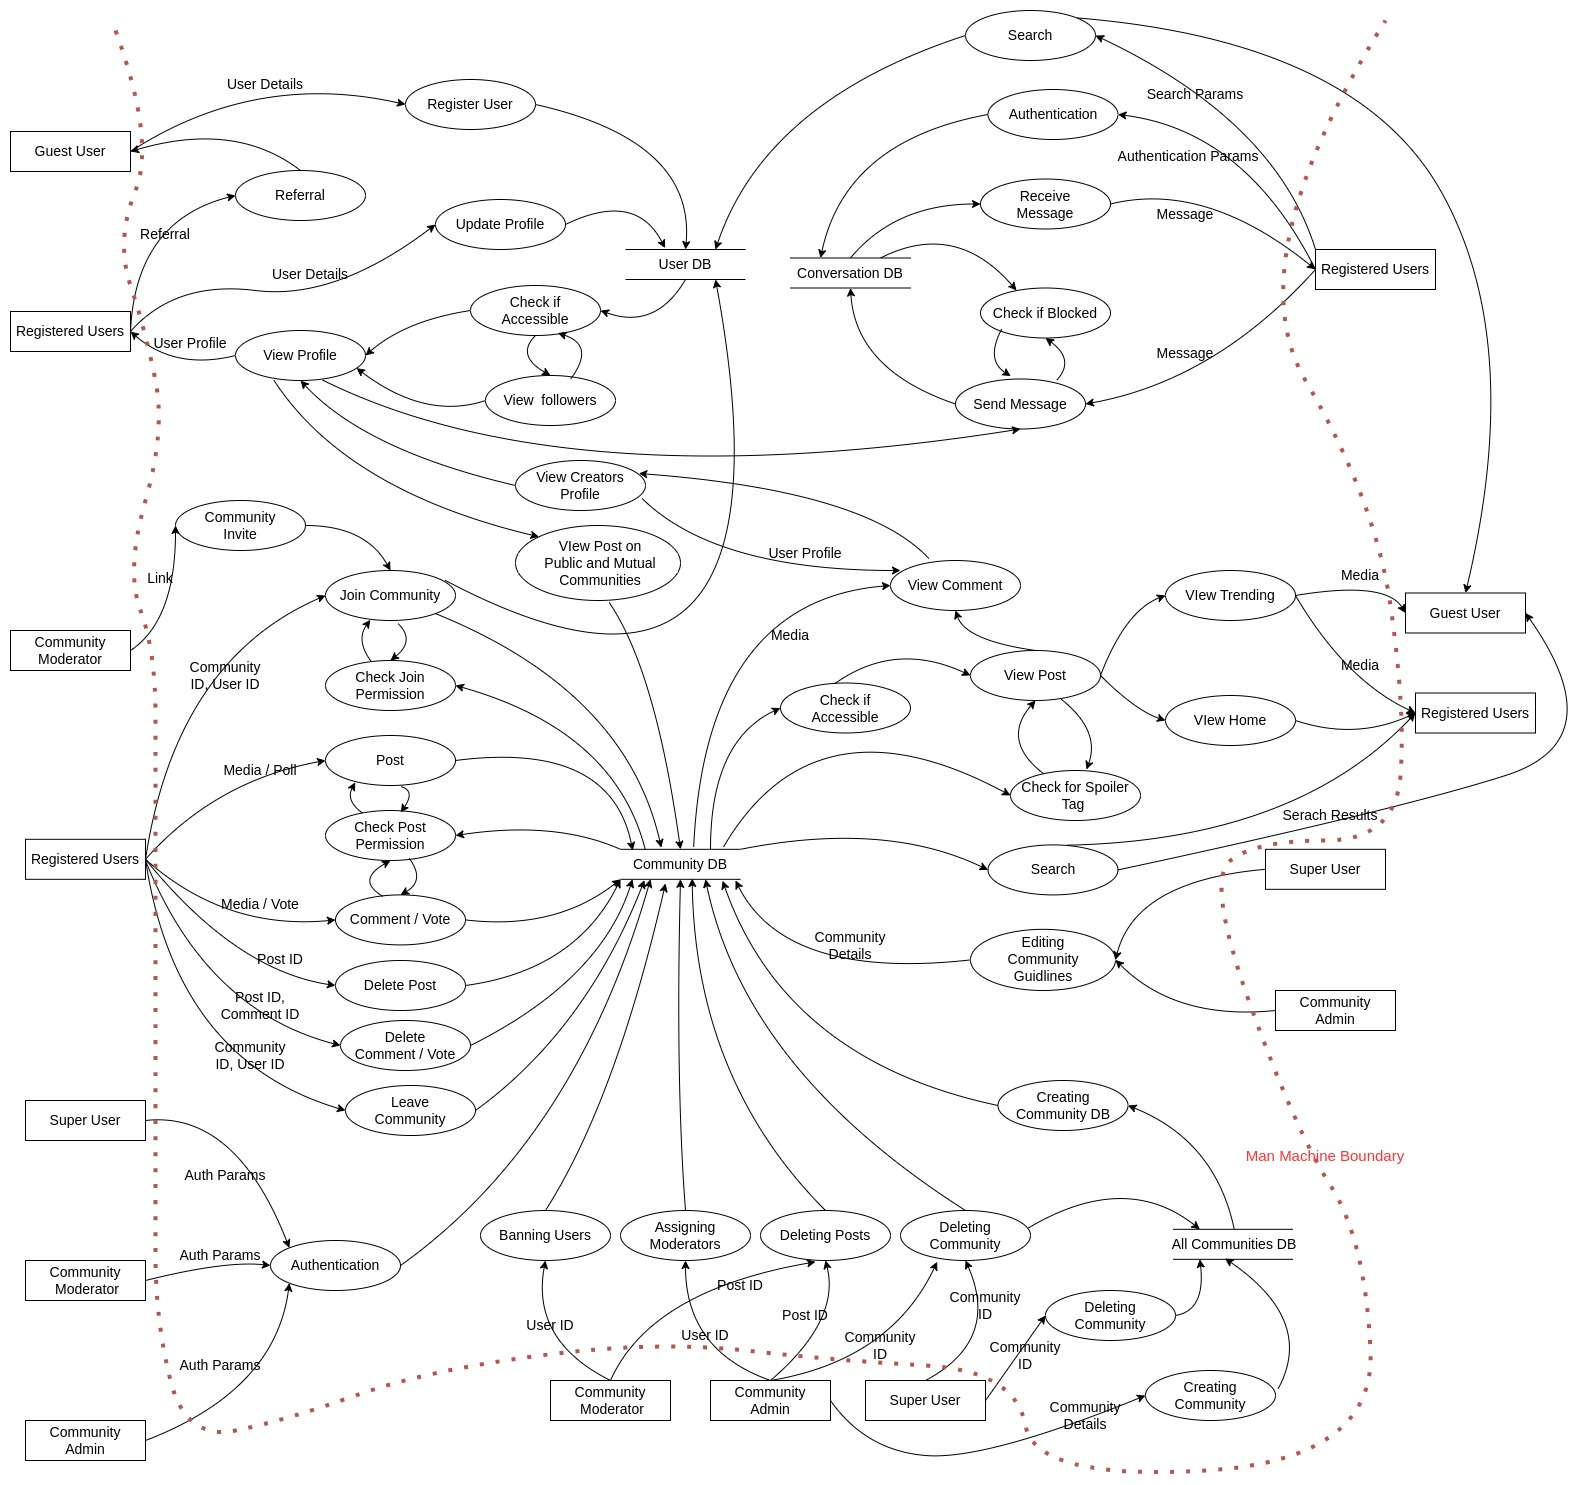
\includegraphics[width = 0.8\textwidth]{./images/dfd_correct.jpeg}
    }
    \caption{Incorrect DFD}
\end{figure}
\begin{figure}[H]
    \centering
    \makebox[\linewidth][c]{\hspace{1cm}
        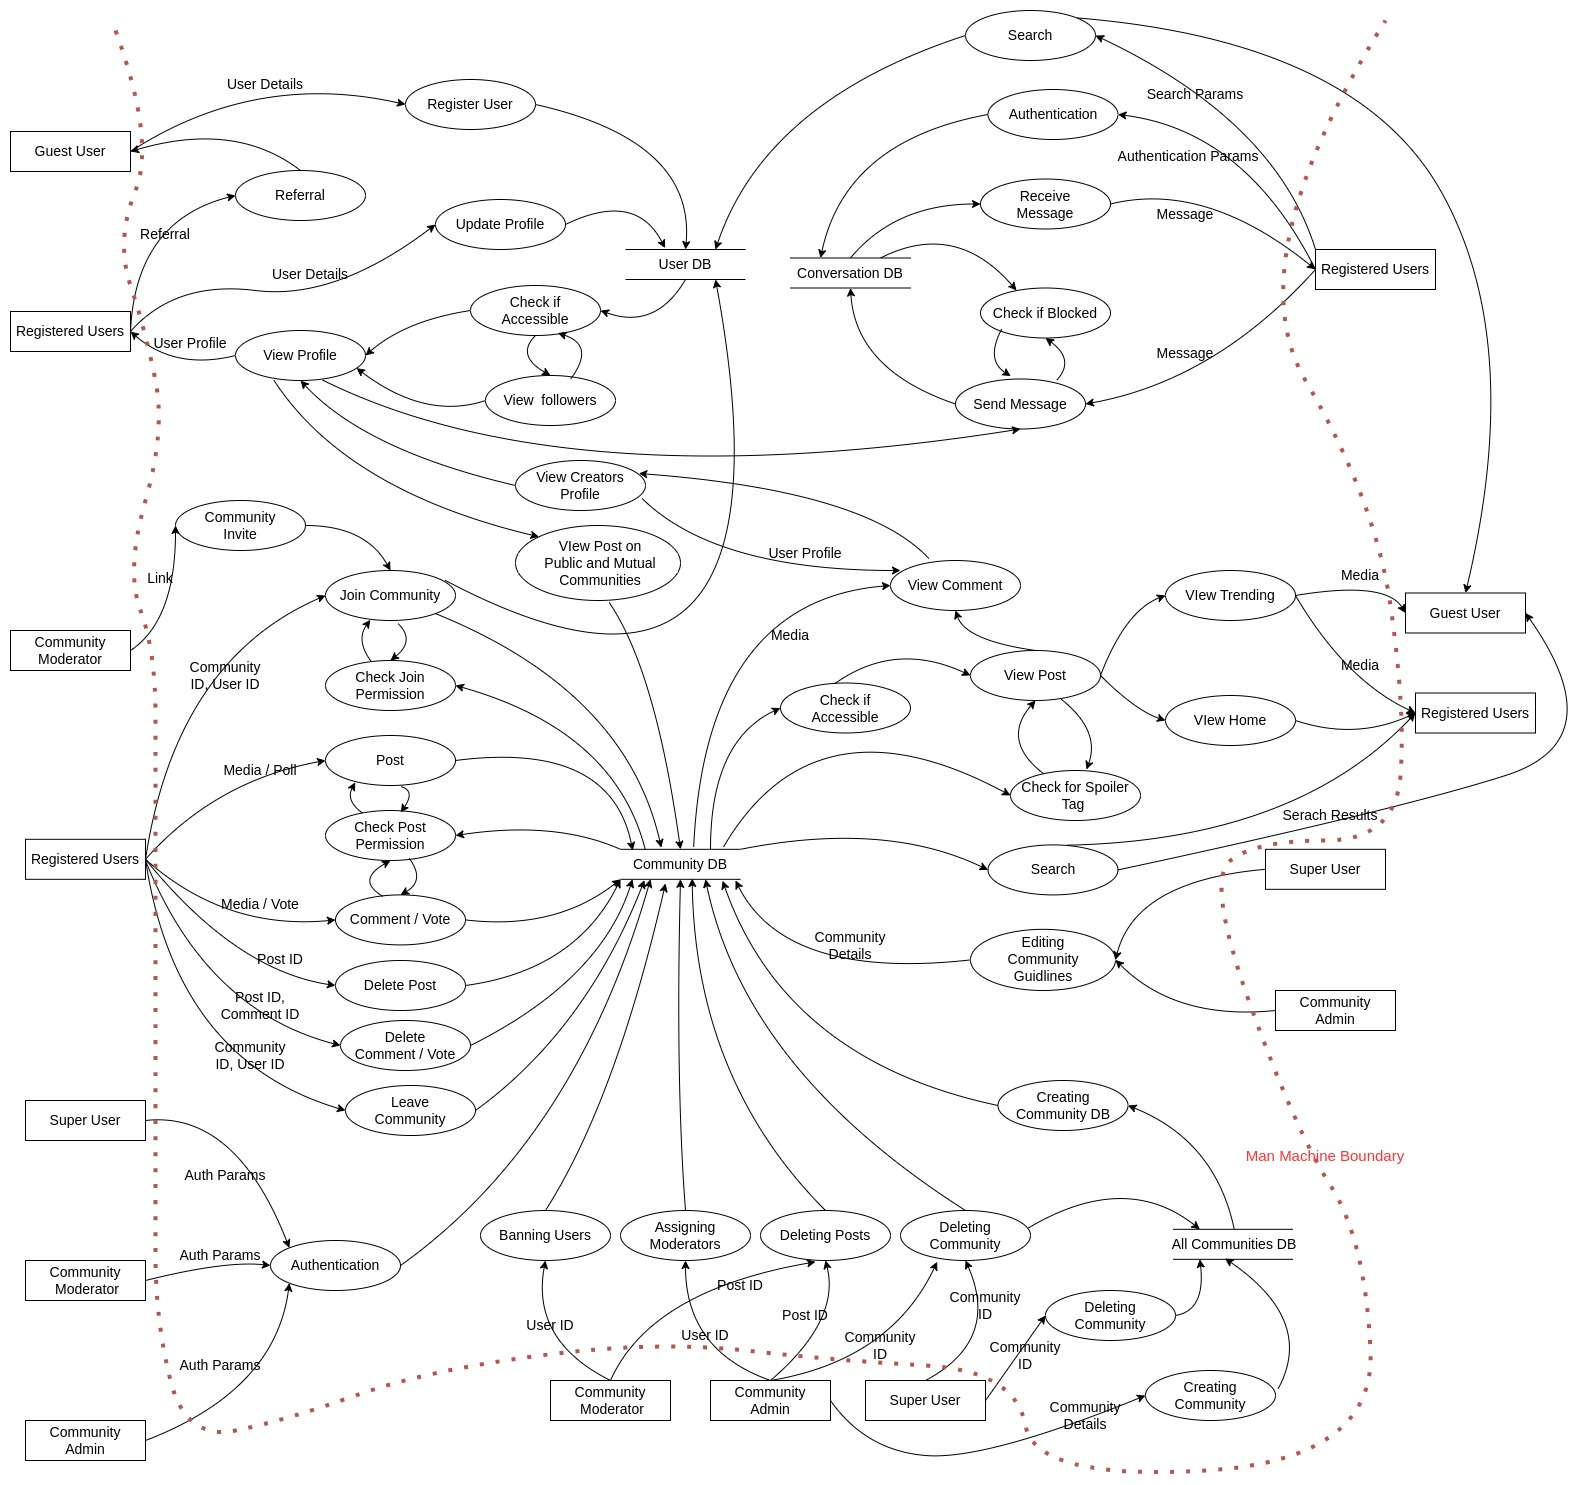
\includegraphics[width = \textwidth]{./images/dfd_correct.jpeg}
    }
    \caption{Correct DFD}
\end{figure}
\begin{itemize}
    \item The below DFD contains the data flow in the system with a man machine boundary
    \item The human part DFD contains only the actors in the system and everything else consists in the machine part
    \item The actors in the system are not exclusive a community moderator is registered user, a community admin is community moderator, a registered user can become a community admin
    \item The DFD consist of these databases : User Database, Conversation Database and Community Database
    \item The data flow from registered user occurs in form of authentication, creating posts, commenting, chatting, deleting, viewing the feed with some restriction regarding communities and user profiles
    \item The data flow from guest user occurs in form registering, viewing trending feed
    \item The data flow in case of community moderator specifically happens in banning users, inviting people to community, deleting posts and comments
    \item The data flow from community admin occurs in creating community, assigning moderators, deleting owned community
    \item The data flow from Super User occurs in deleting communities maintaining community guidelines
\end{itemize}
\subsection{Comparing the two DFDs}
\begin{itemize}
    \item There exist many differences in two DFD discussed earlier and the second DFD is more efficient and reduces redundancy in the system
    \item The main difference would be that the data flow is not that modular
    \item Some dataflows are unnecessary or even loopholes in the system like community moderators assgning new community moderators
    \item The dataflow to check the communites joined by an user requires to search through all the community DB as this is not stored in user database in the first inefficient DFD
    \item Some functionalities like viewing someones profile by seeing their comment or post is not possible in first inefficient DFD
    \item Also Functionality like able to view posts on common communities by visiting a user's profile is missing in the first inefficient DFD
    \item Function for blocking users, viewing community home pages is not available in the first inefficient DFD
\end{itemize}
\section{Function Point Analysis}
\begin{table}[H]
    \centering
    \begin{tabular}{|p{3cm}|p{3cm}|p{3cm}|p{3cm}|}
        \hline
        \textbf{Function Type}  & \textbf{Simple} & \textbf{Medium} & \textbf{Complex} \\
        \hline
        External Input          & 3               & 4               & 6                \\
        \hline
        External Output         & 4               & 5               & 7                \\
        \hline
        External Inquiry        & 3               & 4               & 6                \\
        \hline
        Internal Logical File   & 7               & 10              & 15               \\
        \hline
        External Interface File & 5               & 7               & 10               \\
        \hline
    \end{tabular}
    \caption{Function Point Complexity Weights}
\end{table}

\subsection{UFP Caluculation}

\begin{itemize}
    \item \textbf{External Input:} Data or control information that comes from outside the application's boundary.
    \item \textbf{External Output:} Data or control information that is sent to outside the application's boundary.
    \item \textbf{External Inquiry:} Input-output combination, where input causes and immediate output and leaves the data intact.
    \item \textbf{Internal Logical File:} A user identifiable group of logically related data that resides entirely within the application boundary and is maintained through external inputs.
    \item \textbf{External Interface File:} A user identifiable group of logically related data that is used for reference purposes only.
\end{itemize}

Now we need to count the number of each of these in our system.\\

\begin{itemize}
    \item \textbf{External Input:}
          \begin{enumerate}
              \item User Login (Simple)
              \item User Signup (Simple)
              \item Entering Referal Code (Simple)
              \item Create a post (Medium)
              \item Create a comment (Simple)
              \item Create a reply (Simple)
              \item Create a community (Medium)
              \item Edit a post (Medium)
              \item Edit a comment (Simple)
              \item Edit a community settings (Medium)
              \item Assign privileges to a user (Medium)
              \item Assign a moderator to a community (Medium)
              \item Edit user settings (Simple)
              \item Edit user profile (Simple)
              \item Join request to a community (Simple)
              \item Voting in a poll (Simple)
              \item Upvote/Downvote a post/comment (Simple)
              \item Chat request (Simple)
              \item Send a message (Simple)
              \item Revealing a post which has a spoiler tag (Medium)
              \item Accepting reports (Simple)
              \item Accepting unban requests (Simple)
              \item Accepting a join request (Simple)
          \end{enumerate}
    \item \textbf{External Output:}
          \begin{enumerate}
              \item Sending a forgot password email (Simple)
              \item Sending a verification email at the time of signup/change in email id. (Simple)
              \item Sending a referral link. (Simple)
              \item Displaying the user-feed. (Complex)
              \item Displaying the trending page. (Complex)
              \item Displaying a post. (Simple)
              \item Displaying a comment. (Simple)
              \item Displaying reports to admin (Simple)
              \item Displaying unban request to admin (Simple)
          \end{enumerate}
    \item \textbf{External Inquiry:}
          \begin{enumerate}
              \item Displaying the user profile. (Complex)
              \item Displaying the community page. (Complex)
              \item Displaying search results. (Complex)
              \item Displaying the chat page. (Medium)
              \item Displaying the user's inbox. (Medium)
              \item Displaying all discussions threads. (Complex)
              \item Displaying followers/following list. (Medium)
              \item Sorting/filtering search results (Complex)
              \item Displaying posts in mutual communities (Complex)
          \end{enumerate}
    \item \textbf{Internal Logical File:}
          \begin{enumerate}
              \item Generating trending posts (Complex)
              \item Generating user feed (Complex)
              \item Generating referrals (Simple)
              \item Filtering user profiles based on user-privacy settings (Medium)
              \item Filtering community posts based on community settings (Complex)
              \item Deleting comments when parent post is deleted (Complex)
              \item Filtering search results based on community settings. (Medium)
              \item Marking posts/comments as deleted when community is deleted (Simple)
          \end{enumerate}
    \item \textbf{External Interface File:}
          \begin{enumerate}
              \item Integration with Google OAuth (Complex)
              \item Integration with GMail (Medium)
          \end{enumerate}
\end{itemize}

\begin{table}[H]
    \centering
    \begin{tabular}{|p{3.2cm}|p{3.2cm}|p{3.2cm}|p{3.2cm}|}
        \hline
        \textbf{Function Type}           & \textbf{Simple-Count} & \textbf{Medium-Count} & \textbf{Complex-Count} \\\hline
        \textbf{External Input}          & 16                    & 7                     & 0                      \\\hline
        \textbf{External Output}         & 7                     & 0                     & 2                      \\\hline
        \textbf{External Inquiry}        & 0                     & 3                     & 6                      \\\hline
        \textbf{Internal Logical File}   & 2                     & 2                     & 4                      \\\hline
        \textbf{External Interface File} & 0                     & 1                     & 1                      \\\hline
    \end{tabular}
    \caption{UFP Calculation Table}
\end{table}
\begin{align}
    \text{UFP} & = 16\times3 + 7\times4 + 0\times6 + 7\times4 + 0\times5 + 2\times7 + 0\times3 + 3\times4 \\\notag &+6\times6 + 2\times7 + 2\times10 + 4\times15 + 0\times5 + 1\times7+ 1\times10\\
               & = 277
\end{align}
\subsection{VAF}
\begin{table}[H]
    \centering
    \begin{tabular}{|c|p{5cm}|p{3cm}|}
        \hline
        \textbf{SR.} & \textbf{General System Characteristics (GSCs)} & \textbf{Degree of Influence} \\\hline
        1            & Data Communications                            & 4                            \\\hline
        2            & Distributed Data Processing                    & 1                            \\\hline
        3            & Performance                                    & 4                            \\\hline
        4            & Heavily Used Configuration                     & 0                            \\\hline
        5            & Transaction Rate                               & 4                            \\\hline
        6            & Online Data Entry                              & 2                            \\\hline
        7            & End-User Efficiency                            & 4                            \\\hline
        8            & Online Update                                  & 1                            \\\hline
        9            & Complex Processing                             & 3                            \\\hline
        10           & Reusability                                    & 4                            \\\hline
        11           & Installation Ease                              & 0                            \\\hline
        12           & Operational Ease                               & 3                            \\\hline
        13           & Multiple Sites                                 & 0                            \\\hline
        14           & Facilitate Change                              & 3                            \\\hline
    \end{tabular}
    \caption{Degree of Influence Table}
\end{table}

\begin{align}
    \text{VAF} & = 0.65 + 0.01\times\Sigma_{i=1}^{14}(\text{Degree of Influece})_i \\
               & = 0.65 + 0.01\times(4+1+4+0+4+2+4+1+3+4+0+3+0+3)                  \\
               & = .99
\end{align}
\subsection{FP Caluculation}
\begin{align}
    \text{FP} & = \text{UFP} \times \text{VAF} \\
              & = 277 \times 0.99              \\
              & = 274.23
\end{align}
Considering that 1 FP corresponds to 50-60 LOC (Lines of Code), we can estimate the total LOC to be around \textbf{14 KLOC to 17 KLOC}.
\end{document}